\documentclass[11pt,a4paper]{article}
\usepackage[margin=24mm]{geometry}
\usepackage[T1]{fontenc}\usepackage[utf8]{inputenc}\usepackage{lmodern}
\usepackage{amsmath,amssymb,booktabs,longtable,array,graphicx,float,xcolor,xurl,hyperref,fancyhdr}
\setlength{\emergencystretch}{2em}
\hypersetup{colorlinks=true,linkcolor=blue!45!black,urlcolor=blue!45!black}
\setlength{\parindent}{0pt}\setlength{\parskip}{6pt}
\pagestyle{fancy}\fancyhf{}\fancyhead[L]{Internet Advertisement Classification}\fancyhead[R]{Statistical report}\fancyfoot[C]{\thepage}\setlength{\headheight}{14pt}
\newcommand{\code}[1]{\texttt{\detokenize{#1}}}
\title{Predicting Internet Advertisements from Image Geometry and Web-Context Features\\\large A grouped benchmark investigation}
\date{}
\begin{document}
\begin{titlepage}\centering
{\Large PROBABILITY AND STATISTICS\\PROJECT REPORT\par}\vspace{18mm}
{\huge\bfseries Predicting Internet Advertisements\par}\vspace{5mm}
{\Large From Image Geometry and Web-Context Features\par}\vspace{8mm}
{\large A reproducible study of the UCI Internet Advertisements dataset\par}\vspace{15mm}
\begin{minipage}{.92\textwidth}
\textbf{Administrative completion required before submission.} The supplied materials do not identify the submitting institution/faculty, course identifier, class, group, instructor, student names or IDs, or member contributions. These must be supplied by the group; they have not been invented. The R code is publicly hosted at \url{https://github.com/hlbathien/internet-advertisements-study}. Section 7 provides the actual local code and source locations.

\begin{tabular}{p{.27\textwidth}p{.61\textwidth}}\toprule
Required cover field & Status\\\midrule
Faculty / institution & Not supplied\\
Course / class / group & Not supplied\\
Instructor & Not supplied\\
Members and student IDs & Not supplied\\
Contribution descriptions & Not supplied; describe actual member work\\\bottomrule
\end{tabular}
\end{minipage}\vfill
\textbf{Language: English}\par
Analysis executed in R; independently checked in Python.\par
\end{titlepage}
\pagenumbering{roman}\tableofcontents\newpage\pagenumbering{arabic}
\section{Data overview and research objectives}
\subsection{Problem, scope, and principal findings}
The task is to predict whether a candidate image on a web page is an advertisement (\code{ad}) or not (\code{nonad}). The supplied file is not an image collection: it is a tabular representation containing image geometry and indicators extracted from surrounding web context. Consequently, this study evaluates classification from supplied features, not visual recognition from pixels.

The selected full-feature ridge logistic model achieved held-out average precision (AP) of 0.863 and ROC AUC of 0.957. At a threshold selected exclusively on validation data, it detected 67 of 84 test advertisements, with 25 false alarms among 542 non-advertisements. Test F1 was 0.761. These results support useful discrimination within this benchmark, but do not establish contemporary-web performance, site-level transfer, or a deployment-ready blocking policy.

\subsection{Provenance and unit of observation}
The local \code{data/add.csv} contains 3,279 rows, 1,558 predictors, one class column, and an extra exported row index. Every predictor and label was compared with the original UCI \code{ad.data} download: numeric values, missingness positions, and labels match in row order. Feature names were recovered in order from \code{ad.names}. The source is credited to Nicholas Kushmerick; the repository identifies the dataset as Internet Advertisements, DOI \href{https://doi.org/10.24432/C5V011}{10.24432/C5V011} [2].

The original study is Kushmerick (1999), \emph{Learning to remove Internet advertisements}, Proceedings of the Third Annual Conference on Autonomous Agents, pp. 175--181, DOI \url{https://doi.org/10.1145/301136.301186}. The source documentation identifies the supplied matrix as its STANDARD encoding and reports historical C4.5rules accuracy above 97\%. That result is not a replication target here: the original evaluation protocol has not been recovered reliably enough for a like-for-like comparison.

One row represents a candidate image described through extracted attributes. Raw pixels, original page identifiers, timestamps for individual observations, site grouping identifiers, and an executable feature-extraction pipeline are not supplied. Sampling and annotation reliability cannot be reconstructed from the available matrix. The dataset is an archival benchmark; its sampling frame is not documented sufficiently to establish representativeness of current web images. The accompanying documentation dates data generation to April--July 1998 and identifies the STANDARD encoding used in the original study, emph{Learning to remove Internet advertisements} (1999). That historical context matters: URL conventions and image templates represented here are not a current-web sampling frame.

The observed class counts are 459 ads (14.00\%) and 2,820 nonads (86.00\%). The accompanying original documentation instead states 458 and 2,821. The actual local and original data agree with each other, so all calculations use the measured counts, not the inconsistent prose. This discrepancy is documented rather than silently corrected in the source.

\subsection{Research questions}
\begin{enumerate}
\item How do the available geometric measurements differ between ad and nonad observations, and what does missingness imply for their interpretation?
\item Do the full context features improve held-out ranking beyond geometry and locality alone?
\item How do ranking, probability quality, and classification trade-offs differ among a majority baseline, ridge logistic models, and a constrained decision tree?
\item How uncertain are the final test estimates when repeated predictor patterns are treated as clusters, and what limits generalization?
\end{enumerate}
The empirical target is performance on withheld predictor-pattern groups from this dataset under the stated partition design. Broader population claims require additional sampling assumptions; this is not a probability sample of today's Internet.

\begin{table}[H]\centering\small
\caption{Predictor families recovered from the original ordered dictionary.}
\begin{tabular}{lrl}\toprule Family & Count & Meaning / representation\\\midrule
Height, width, aspect ratio & 3 & Continuous geometric measurements\\
Local & 1 & Binary locality indicator; exact operational rule unavailable\\
URL terms & 457 & Binary phrase indicators from image URL\\
Original-URL terms & 495 & Binary indicators in source code{origurl} family\\
Anchor-URL terms & 472 & Binary phrase indicators from anchor URL\\
Alt-text terms & 111 & Binary phrase indicators from alternative text\\
Caption terms & 19 & Binary phrase indicators from nearby/caption context\\\midrule
Total & 1,558 & Three continuous and 1,555 binary predictors\\\bottomrule
\end{tabular}\label{tab:families}
\end{table}
Table~\ref{tab:families} shows that contextual indicators dominate dimensionality. A phrase indicator denotes the source encoding, not a directly verified linguistic or causal mechanism. The dictionary names geometry but does not provide explicit units; numerical dimensions are therefore reported in source units, rather than assigning undocumented units.
\section{Statistical and predictive background}
\subsection{Binary outcomes, loss, and regularized logistic regression}
Let $Y_i=1$ denote ad and $X_i$ the observed feature vector. Logistic regression models
\[p_i=P(Y_i=1\mid X_i)=\{1+\exp[-(\beta_0+X_i^T\beta)]\}^{-1}.\]
For standardized fitting inputs $Z$, write $p_i=\operatorname{logit}^{-1}(\gamma_0+Z_i^T\gamma)$. Ridge regression estimates $\gamma$ by minimizing the mean binomial negative log-likelihood plus a quadratic penalty,
\[ -\frac1n\sum_i\{y_i\log p_i+(1-y_i)\log(1-p_i)\}+\frac\lambda2\sum_j\gamma_j^2. \]
Here $\gamma$ denotes fitting-scale slopes and $\beta$ denotes the back-transformed slopes reported later. The intercept is not penalized. In \code{glmnet}, ridge corresponds to $\alpha=0$ and standardization is performed using the fitting sample [1]. Regularization is important because the predictor count is large relative to the training sample and binary indicators can be rare or correlated. A finite ridge solution is more suitable than attempting unrestricted maximum-likelihood inference across all 1,558 predictors.

This is a predictive model: coefficients describe conditional fitted associations, not causal effects. Standard unpenalized coefficient p-values are not supplied for this penalized, tuned model. Nonlinearity and interactions may be inadequately represented by a linear logit; regularization does not prove model correctness or probability calibration.

The geometry model uses $\log(1+x)$ transformations of height, width, and aspect ratio, the locality indicator, and four missingness indicators. The full model adds all context indicators. This comparator is technically geometry-plus-locality; the shorter label ``geometry'' refers to that explicit feature set.

\subsubsection{Why this model and scale?}
The model is linear in the \emph{log odds}, $\log\{p/(1-p)\}$, not in probability. A one-unit increase in a transformed predictor changes fitted odds by $\exp(\beta_j)$, holding the other encoded inputs fixed. A positive score contribution raises probability most near the middle of the logistic curve and less near its extremes. This distinction explains why coefficient signs alone do not imply a useful classification threshold.

The log1p transform compresses large geometric values while retaining zero. A change from source width $w_1$ to $w_2$ contributes $\beta_w\log\{(1+w_2)/(1+w_1)\}$ to the geometry-model logit. It therefore makes proportional differences more comparable across scales, without assuming that geometry is normally distributed. It is a modeling choice, not a normality correction; logistic regression does not require normally distributed predictors.

With $z_{ij}=(x_{ij}-\mu_j)/s_j$, the fitting-scale ridge penalty shrinks standardized slopes $\gamma_j$. Back-transformation gives $\beta_j=\gamma_j/s_j$ and adjusts the intercept. Thus its penalty on the reported-scale slopes is proportional to $\sum_j s_j^2\beta_j^2$, not an equal penalty on every raw-scale coefficient. For a binary feature of frequency $q$, $s_j^2=q(1-q)$: a large raw slope for a rare indicator need not mean a large standardized contribution. Strong shrinkage approaches a near-constant probability; weak shrinkage permits a more variable fitted surface. The selected penalty trades training fit against complexity through development data, rather than proving that the linear-logit representation is true.


\subsection{Constrained classification tree}
A classification tree partitions feature space through sequential splits and assigns probabilities using terminal-node class frequencies. For binary classes, the default Gini impurity at a node with ad fraction $q$ is $G(q)=2q(1-q)$. A candidate split gains $G(q)-\{n_LG(q_L)+n_RG(q_R)\}/n$. This is a local improvement, not the AP criterion used to compare the completed trees. Sequential splits can express interactions: a URL indicator can matter in one width region and not another. Depth and minimum-node constraints limit that flexibility but do not establish stability. The \code{rpart} implementation uses classification splitting and a complexity parameter $cp$; larger $cp$ discourages splits with small improvements [3]. The tree here has maximum depth five and minimum split size 20. It provides a nonlinear comparator without building an extensive model-search exercise. Leaf probabilities are discrete and can be poorly calibrated; a strong classification threshold need not imply strong ranking across the entire score range.

\subsection{Metrics and decision thresholds}
For counts TP, FP, FN and TN, with ad as positive,
\[\mathrm{precision}=\frac{TP}{TP+FP},\quad \mathrm{recall}=\frac{TP}{TP+FN},\quad F_1=\frac{2TP}{2TP+FP+FN}.\]
Balanced accuracy averages sensitivity and specificity. Accuracy alone is insufficient: predicting every case as nonad already scores about 86\% here while detecting no ads. When no positive predictions occur, precision is recorded as zero by reporting convention, not as an estimated conditional probability.

ROC AUC is the probability that a random positive receives a higher score than a random negative, counting ties as one half. AP aggregates precision over recall increments at distinct score thresholds:
\[\mathrm{AP}=\sum_k(R_k-R_{k-1})P_k.\]
Ties are pooled before computing increments. AP is not trapezoidal PR area [4], and depends on class prevalence. A constant-score classifier has AP equal to observed positive prevalence. The Brier score $n^{-1}\sum_i(p_i-y_i)^2$ evaluates squared probability error; smaller is better.

Model selection maximizes training cross-validation AP. The final decision threshold maximizes validation F1, choosing the highest threshold if tied. AP selects ranking ability, whereas F1 selects one operating point; their preferences need not coincide. No business cost ratio is supplied, so this threshold is an explicit analytical convention, not an optimal ad-blocking policy. False blocking of useful content and missed advertisements may have very different costs.

\subsection{Metric meaning and prevalence}
A ranking asks which candidate to inspect first; a probability asks how often similarly scored candidates are ads; a decision asks whether the consequences justify acting. AP evaluates the first, Brier assesses squared probability error, and F1 summarizes one decision set. For a four-record illustration with descending labels $(1,0,1,0)$, positive records arrive at recalls $1/2$ and $1$ with precisions $1$ and $2/3$, giving AP $\tfrac12(1)+\tfrac12(2/3)=5/6$. Moving probabilities without changing their order leaves AP unchanged but can change Brier and thresholded decisions.

If sensitivity is $s$, false-positive rate is $f$, and ad prevalence is $\pi$, precision equals
\[\frac{\pi s}{\pi s+(1-\pi)f}.\]
The frozen test rates $s=67/84$ and $f=25/542$ give observed precision .728 at prevalence $84/626$, but about .149 at hypothetical prevalence .01. This is an algebraic scenario assuming unchanged class-conditional rates, not external validation. Benchmark ranking alone cannot establish positive predictive value in another environment.

\subsection{Exploratory distribution comparisons and uncertainty}
The rank comparison $U/(n_1n_0)$ summarizes the fraction of observed ad--nonad pairs for which the ad has a larger value, counting ties as one half. This is a descriptive, row-weighted measure of separation, not automatically a median effect. Missing measurements are excluded separately for each variable. Because repeated representations and unobserved website dependence undermine an independent-row reference distribution, geometry significance tests are not used as evidence in this report. The analysis exports descriptive rank separation without independent-row significance tests.

Predictive inference instead uses an explicit working model: representation clusters are exchangeable draws from a benchmark-like generating mechanism, and each cluster contributes all of its rows. The target weights candidate-image records, rather than unique signatures equally. More precisely, the inferential target is the AP difference between these two fixed scoring functions under the row distribution induced by independent draws of representation clusters from the working population. It is not the difference between algorithms retrained on new datasets. The observed finite-test difference is a separate descriptive quantity; the interval concerns sampling that test composition under this model. Under that model a population metric is a functional of cluster-level counts and scores; for example recall is $E[TP_g]/E[TP_g+FN_g]$, where $g$ denotes a cluster. The ratio is estimated by totals over the sampled clusters. This model permits arbitrary dependence within a signature but assumes independence across signatures, an assumption not established for shared websites. It is a conditional modeling abstraction, not a claim about a probability sample of Internet images. The bootstrap allows cluster composition and prevalence to vary; it is not design-based inference conditional on the fixed stratified allocation.

For final predictive uncertainty, 1,000 bootstrap samples resample entire test predictor-pattern groups with replacement. The number sampled equals the 484 observed test groups; the row count can vary because group sizes differ. Each replicate recomputes the whole metric, rather than averaging per-group F1 or AP. For the AP contrast, $\Delta_b=\mathrm{AP}_{full,b}-\mathrm{AP}_{geometry,b}$ uses the same sampled groups in both terms, preserving their shared easy and difficult cases. All rows in a selected group are retained, and a repeatedly selected group contributes repeatedly. Percentile endpoints at 2.5\% and 97.5\% quantify conditional test-sample uncertainty. Training, parameter selection, and threshold selection are not repeated; intervals do not include their instability or unobserved domain clustering.
\section{Data preprocessing and evaluation design}
\subsection{Observed integrity checks}
The exported index runs consecutively from 0 to 3,278 and is removed before modeling. It is not a predictor. Class strings are trimmed, terminal punctuation is normalized conceptually, and ad is encoded as one. The original ordering places many ads together; neither an order-based split nor using the index would be appropriate.

Numeric parsing recognizes whitespace-padded question marks as unknown values. Missingness occurs in height (903 rows), width (901), aspect ratio (910), and locality (15). At least one geometry value is absent in 910 rows; 920 rows have any missing predictor. Thus 28.06\% of rows have missing data. The source's ``unknown'' interpretation is retained; unknown is not converted to zero.

All observed non-geometric predictors are binary. Their mean observed activation rate is 0.821\%, illustrating sparsity. No globally constant source feature was found. Valid extreme dimensions are retained: an outlier rule is not evidence of an incorrect image size. The original file remains unchanged.

\subsection{Duplicate-pattern audit}
There are 2,420 distinct predictor patterns and 859 repeated rows beyond their first occurrences (26.20\% of rows). Pattern identity includes all predictors and missingness positions but excludes labels and the exported index. These are identical \emph{representations}; the data do not establish whether they are literally the same image or page.

Three patterns have conflicting labels: group sizes and ad counts are respectively $(49,1)$, $(3,2)$, and $(2,1)$. The smallest unavoidable number of errors for any deterministic classifier that sees only this feature representation is three on these observed rows. This is an in-sample representation constraint, not an estimate of a population Bayes error. Conflicting labels are not changed or deleted. The first two conflicting groups fall in training and the third in validation; none is in the test partition.

A random row split could place indistinguishable representations on both sides of evaluation. To avoid that, all rows with the same predictor pattern are assigned to the same partition and training fold. Different patterns can nevertheless share pages or domains: unavailable identifiers prevent stronger leakage controls.

\begin{table}[H]\centering
\caption{Fixed grouped partition, with class counts measured after allocation.}
\begin{tabular}{lrrrr}\toprule
Partition & Rows & Patterns & Ads & Nonads\\\midrule
Train & 1984 & 1452 & 288 & 1696\\
Validation & 669 & 484 & 87 & 582\\
Test & 626 & 484 & 84 & 542\\
\bottomrule\end{tabular}
\label{tab:split}
\end{table}
Table~\ref{tab:split} reflects approximately 60/20/20\% of patterns, not exactly those percentages of rows. Groups are stratified by majority label (ties assigned to ad); within each stratum their allocation is randomized. The delivered split assignments identify the evaluation sample; robustness to alternative allocations is not estimated. Labels are used for stratification, not to compute feature transformations. The partition is a designed benchmark comparison, not a guarantee of naturally occurring deployment prevalence.

\subsection{Training-only transformations and model selection}
The three geometry variables undergo $\log(1+x)$ transformation. Four missingness indicators are appended. Medians are learned separately from each training fold, and used to fill corresponding fold-held-out data. For binary locality, the median is a modal value here. No class balancing, oversampling, or synthetic rows are introduced.

The five-fold training procedure keeps identical patterns together. Ridge models examine 25 logarithmically spaced penalties from $10^2$ to $10^{-4}$; the tree examines $cp\in\{.001,.005,.01,.02,.05\}$. Each model's parameter maximizes the unweighted mean of five fold AP values. The winning model family is also selected by this training-only criterion. Mean fold AP need not equal AP of pooled out-of-fold predictions.

After selection, each comparator is fit on the full training partition. Medians and ridge scaling remain training-derived. The selected model's threshold is selected on validation data only, then frozen before test metrics are generated. Training and validation are \emph{not} merged for a new final fit; this preserves the exact fitted model associated with the selected threshold. The model-selection CV scores are development scores, not unbiased final-performance estimates.

\subsection{Reproducibility}
The delivered split assignments, fold IDs, fitted models, predictions, and analysis scripts identify the actual experiment. Diagnostic analyses added after inspecting test results are labeled as post-evaluation descriptions and do not change the fitted model or threshold.
\section{Descriptive statistics}
\begin{table}[H]\centering\small
\caption{Observed geometry by class: median [first quartile, third quartile], excluding unknown values.}
\begin{tabular}{llrrr}\toprule
Variable & Class & Observed $n$ & Missing $n$ & Median [Q1,Q3]\\\midrule
Height & nonad & 1990 & 830 & 43.000 [23.000, 90.000]\\
Height & ad & 386 & 73 & 60.000 [60.000, 60.000]\\
Width & nonad & 1992 & 828 & 101.000 [73.000, 150.000]\\
Width & ad & 386 & 73 & 460.000 [126.000, 468.000]\\
Aratio & nonad & 1983 & 837 & 1.724 [1.000, 4.345]\\
Aratio & ad & 386 & 73 & 7.800 [2.222, 7.800]\\
\bottomrule\end{tabular}
\label{tab:desc}
\end{table}
Table~\ref{tab:desc} shows strong concentration at particular ad dimensions, consistent with repeated standardized representations in this benchmark. Ads tend to be wider and have larger aspect ratios among observed measurements. Their height has a degenerate interquartile range at 60, so an ordinary symmetric-normal description would hide important structure. Observed height means are 67.44 for ads and 63.36 for nonads; a small mean difference coexists with markedly different distributions.

Missingness is class-associated descriptively: height is unknown for 15.90\% of ads versus 29.43\% of nonads. Excluding every incomplete row would therefore change class composition and discard over a quarter of the data. Missingness indicators allow a predictive model to use availability information, but that information could shift when a different extractor or website population is used.

\begin{figure}[H]\centering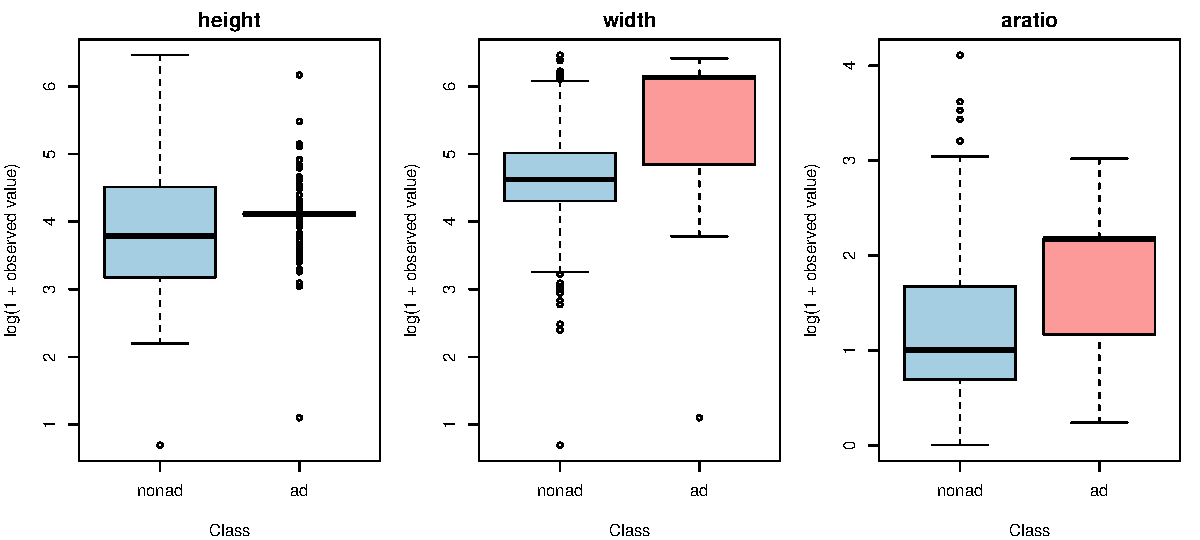
\includegraphics[width=\textwidth]{../analysis/results/distributions.pdf}
\caption{Class-conditional geometry on a log(1+value) scale; unknown values omitted.}\label{fig:geometry}\end{figure}
Figure~\ref{fig:geometry} emphasizes skewness, ties, and distributional overlap. Width and aspect ratio distinguish groups more clearly than height, but no single geometric cutoff perfectly separates the classes. The plots describe the full dataset; they were generated for reporting after the fixed model specification and are not used to select variables or tune the models.

The binary locality mean is 0.775 for observed ads and 0.766 for observed nonads, much less separated than width. The feature dictionary's 1,554 text/context indicators offer many potential distinctions, but high dimension and sparse activation make unregularized exploratory significance scanning particularly prone to instability. No mass screening of these indicators is used to select the model.
\subsection{Context-feature distributions and training support}
\begin{table}[H]\centering
\caption{Mean active context indicators per record, by class, over the supplied dataset.}
\begin{tabular}{lrr}\toprule
Family & Nonad & Ad\\\midrule
url & 3.612 & 3.900\\
origurl & 3.719 & 2.699\\
ancurl & 2.655 & 10.340\\
alt & 0.696 & 2.242\\
caption & 0.089 & 0.383\\
\bottomrule\end{tabular}
\label{tab:context}
\end{table}
Table~\ref{tab:context} reveals that anchor-URL and alternative-text encodings are much more active among ads. These are counts of encoded indicators, not word counts or independent pieces of evidence: overlapping phrases can activate together. The summaries were computed after evaluation for interpretation and were not used to select features. They do not attribute the prediction gain to individual families; that would require a separately specified ablation analysis.

In training, 18 of 1,555 binary predictors never activate, and 241 activate at most five times. Ten test rows activate a binary feature absent from training. Such features cannot have their positive-state effect learned from that training sample. Global nonconstancy therefore does not establish useful training support. Rare terms and overlapping URL phrases also make raw coefficient magnitude a poor stand-alone importance measure.

All 2,369 complete geometry records satisfy aspect ratio approximately equal to width divided by height, within absolute difference 0.00011. Aspect ratio is consequently a derived representation, not an independently manipulable measurement. The log1p transformations do not make these columns exactly linearly dependent, but an interpretation that varies ratio while holding both dimensions fixed would be physically incoherent.

\subsection{Observed training geometry separation}
\textbf{Objective.} Quantify observed training separation without assuming independent rows for significance testing.
\begin{table}[H]\centering\small
\caption{Descriptive training geometry separation; no population significance claim.}
\begin{tabular}{lrrr}\toprule
Feature & Observed ad/nonad $n$ & Ad/nonad medians & Rank separation\\\midrule
height & 242 / 1223 & 60.000 / 40.000 & 0.640\\
width & 242 / 1224 & 468.000 / 100.000 & 0.841\\
aratio & 242 / 1218 & 7.800 / 1.649 & 0.708\\
\bottomrule\end{tabular}
\label{tab:infer}
\end{table}
\textbf{Result.} Width has the largest observed rank separation (Table~\ref{tab:infer}): an observed ad--nonad pair has the ad wider in about 84.1\% of comparisons, with ties counted as one half.

\textbf{Interpretation.} These are empirical effects, weighted by repeated rows and conditional on available measurements. They do not establish a population median difference or remove website dependence. A first-row-per-signature label reduction is not used for inference because conflicting signatures make that reduction arbitrary.

\textbf{Conclusion.} Geometry is associated with class in the observed training sample, especially width. Predictive value must be assessed through the withheld evaluation, not inferred from a small p-value.

\section{Inferential and predictive results}
\subsection{Model selection: objective, result, interpretation, conclusion}
\textbf{Objective.} Choose a ranking model without using test outcomes. All model families and grids are specified in Section 3; no further model search followed the final test evaluation.
\begin{table}[H]\centering
\caption{Training grouped cross-validation selection, using mean fold average precision.}
\begin{tabular}{lrrrr}\toprule
Model & Parameter & Mean AP & Fold SD & Fold range\\\midrule
geometry ridge & 1.0000 & 0.5944 & 0.0999 & 0.4660--0.7009\\
full ridge & 0.5623 & 0.9196 & 0.0176 & 0.9045--0.9479\\
tree & 0.0010 & 0.7913 & 0.1199 & 0.6348--0.9362\\
\bottomrule\end{tabular}
\label{tab:cv}

The fold SD describes variation across these particular folds; it is not a standard error from independent trials. Tree performance varies substantially more than the full ridge in this development comparison. Sixteen ridge penalties are within 0.01 mean AP of the selected full-model value, so the precise selected penalty should not be interpreted as a sharply determined scientific optimum.
\end{table}
\textbf{Result.} Figure~\ref{fig:development} displays the recorded training and validation searches. Fold envelopes are ranges, not confidence bands. The full-feature ridge model wins the training-CV AP criterion recorded in the analysis (Table~\ref{tab:cv}). The tree's chosen complexity is at the least-pruned grid boundary, so the study does not claim to have exhausted tree performance. For each family, the available grid is a finite comparison, not a global optimum search.

\textbf{Interpretation.} Context features appear useful for ranking beyond geometry/locality. Unequal search grids and the limited tree specification mean this is not a definitive comparison of all possible algorithms. Ridge scaling uses fitting-sample variance, including for rare binary indicators; this changes the effective shrinkage of rare features.

\textbf{Conclusion.} Freeze full-feature ridge as the primary ranking model. A different choice of primary utility, such as F1 at 0.5 or false-positive cost, could favor a different model. Test outcomes must not be used to retroactively redefine that criterion.

\subsection{Development behavior}
\begin{figure}[H]\centering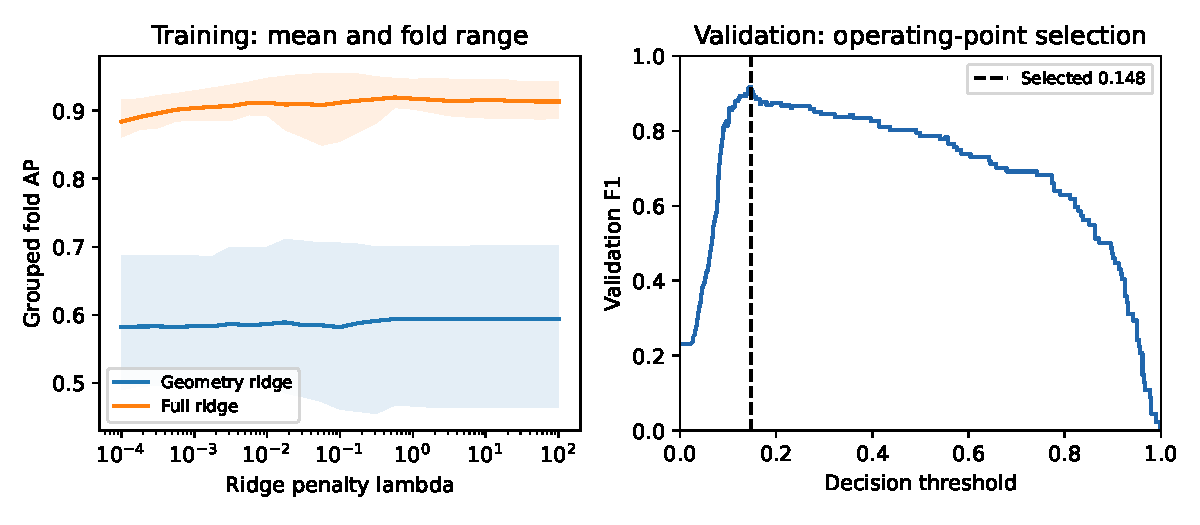
\includegraphics[width=\textwidth]{../analysis/results/development.pdf}
\caption{Recorded development searches: ridge mean fold AP with min--max fold envelopes, and validation F1 over full-ridge thresholds.}\label{fig:development}\end{figure}
Figure~\ref{fig:development} shows how penalty strength changes fit and how the chosen operating point sits on the validation threshold response. Shading is a fold range, not a confidence band. The left panel uses training CV and the right uses validation only; neither adds test-derived tuning. A broad near-best penalty region means the selected numerical penalty is not a sharply identified scientific optimum.

\subsection{What the fitted models actually do}
Let $h,w,r$ denote the imputed log1p geometry values, $l$ the imputed locality, and $m_h,m_w,m_r,m_l$ the four missingness flags. On the original transformed feature scale, the compact comparator has fitted logit
\begin{align*}
\widehat\eta=-3.02745+0.06738h+0.17689w+0.15033r-0.00161l\\-0.05220m_h-0.05213m_w-0.05370m_r+0.24059m_l
\end{align*}

This equation shows why a ranking score need not cross 0.5 even when groups differ descriptively: the intercept and regularized contributions jointly determine the probability. Coefficients refer to transformed, imputed features and are not causal effects.

The fitted tree has seven splits and eight leaves. Its first split is at log1p width 6.053181, corresponding to source width about 424.46; its wider branch splits again near source width 484.92. In the narrower branch, indicators corresponding to \code{ancurl*com}, \code{ancurl*click}, \code{url*ads}, \code{url*ad}, and \code{ancurl*home} distinguish leaves. A wide-image leaf contains 132 training cases with estimated ad probability .9773. The largest low-score leaf contains 1,714 cases with estimated probability .0280. These are training proportions, not externally validated rule probabilities; sparse leaves can be unstable.

The full ridge has 1,544 nonzero fitted slopes. Ridge shrinks rather than generally selects variables, so this count is not evidence of 1,544 independent discoveries. The concrete feature-signature failure below illustrates behavior more directly than a ranking of raw coefficient magnitudes.

\begin{figure}[H]\centering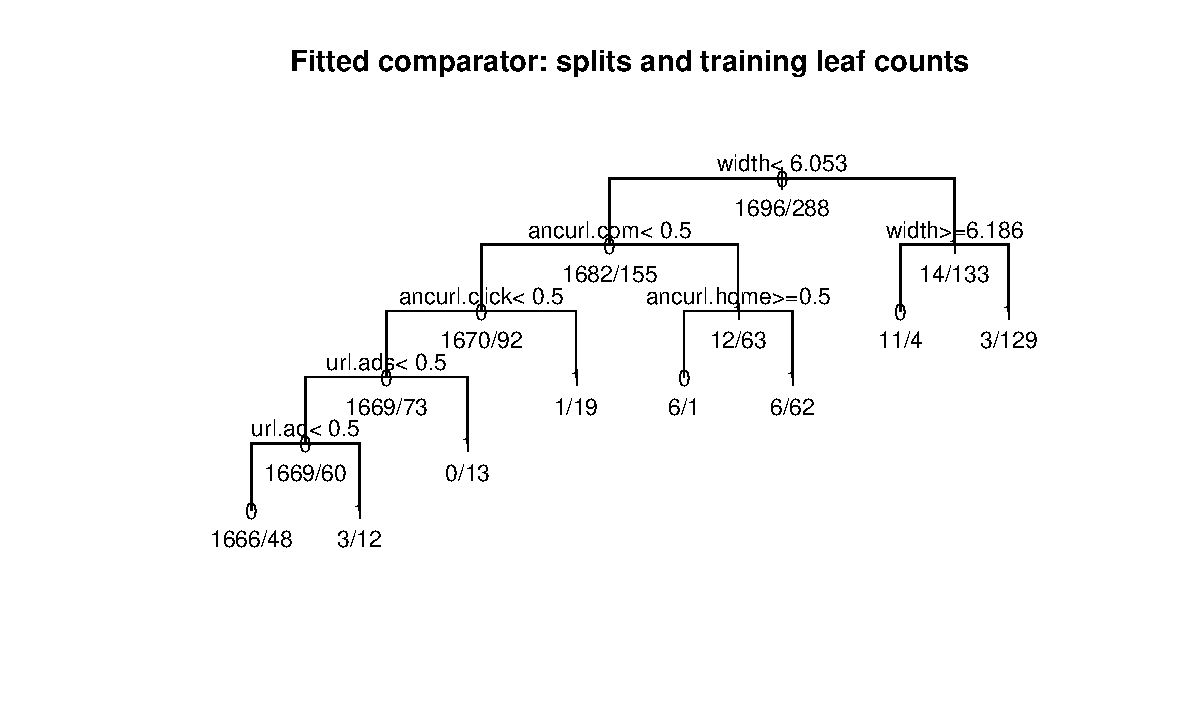
\includegraphics[width=\textwidth]{../analysis/results/tree.pdf}
\caption{Actual fitted tree with transformed-width splits and training class counts at leaves.}\label{fig:tree}\end{figure}
Figure~\ref{fig:tree} displays the interaction of width and URL conditions described above. Width is on the log1p scale; leaf counts describe training support, not independent validation.

\subsection{Threshold selection and final test evaluation}
\textbf{Objective.} Quantify held-out prediction and the operating-point trade-off after selecting the model. Validation F1 is maximized at threshold 0.1481484, yielding validation F1 0.9176. This is a tuned development result, not final evidence of generalization.

\begin{table}[H]\centering\small
\caption{Held-out test results; ad is positive. Model selection did not use this table.}
\begin{tabular}{lrrrrrr}\toprule
Model / operating point & Accuracy & Precision & Recall & F1 & ROC AUC & AP\\\midrule
Always nonad & 0.8658 & 0.0000 & 0.0000 & 0.0000 & 0.5000 & 0.1342\\
Geometry ridge, .5 & 0.8658 & 0.0000 & 0.0000 & 0.0000 & 0.7626 & 0.4626\\
Full ridge, .5 & 0.9457 & 0.9808 & 0.6071 & 0.7500 & 0.9569 & 0.8625\\
Tree, .5 & 0.9553 & 0.9118 & 0.7381 & 0.8158 & 0.8723 & 0.7217\\
Full ridge, tuned & 0.9329 & 0.7283 & 0.7976 & 0.7614 & 0.9569 & 0.8625\\
\bottomrule\end{tabular}
\label{tab:test}
\end{table}
\textbf{Result.} The final tuned ridge correctly identifies 67 ads and 517 nonads, missing 17 ads and falsely flagging 25 nonads. Balanced accuracy is 0.8757; specificity is 0.9539. The raw test accuracy is lower than that of the tree, and the tree also has higher test F1 at its fixed 0.5 threshold (Table~\ref{tab:test}). Full ridge nevertheless has better ranking AP and ROC AUC in this comparison.

\textbf{Interpretation.} There is no uniformly best model across metrics. Geometry ridge ranks ads above nonads moderately well but makes no ad predictions at 0.5: discrimination and a fixed decision threshold are different questions. Lowering full-ridge's threshold raises recall from 0.607 to 0.798 while reducing precision from 0.981 to 0.728. A user-facing blocking system might prefer higher precision; F1 does not encode that preference.

\textbf{Conclusion.} Full-context information materially improves held-out ranking over the geometry/locality comparator. The chosen threshold provides a reproducible example of an operating point, not evidence that automatic blocking is safe or economically optimal. The drop from validation F1 0.918 to test F1 0.761 shows substantial development-to-test variation; possible contributors include threshold selection, finite positive counts, and clustered sample composition. Their separate contributions are not identified here.

\begin{figure}[H]\centering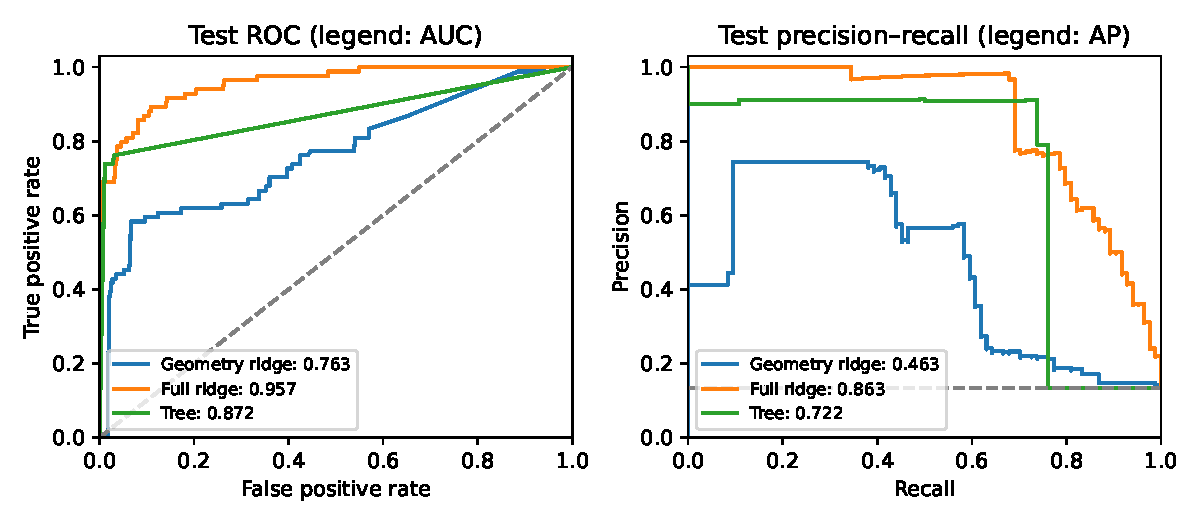
\includegraphics[width=\textwidth]{../analysis/results/performance.pdf}
\caption{Held-out ranking curves for all three fitted comparators. Legends report AUC and AP; dashed lines show random-ranking ROC and test-prevalence PR baselines.}\label{fig:curves}\end{figure}
Figure~\ref{fig:curves} shows the full ridge's stronger overall ranking relative to geometry and the tree, but does not imply superiority at every recall or operating point. The tree has relatively few distinct leaf probabilities, hence a coarse curve. Tied scores enter together; AP .8625 is the sum over recall increments, not the trapezoidal area of a smoothed line. The PR display exposes false alarms among retrieved candidates more directly than ROC when nonads are common.

\begin{figure}[H]\centering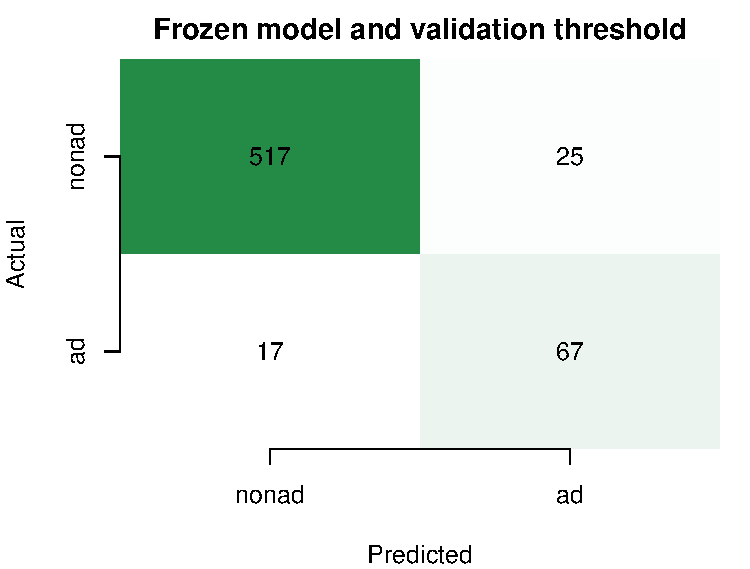
\includegraphics[width=.65\textwidth]{../analysis/results/confusion.pdf}
\caption{Test confusion counts at the validation-selected threshold 0.1481484.}\label{fig:confusion}\end{figure}
Figure~\ref{fig:confusion} makes the remaining errors explicit: 25 false alarms and 17 misses. The 84-positive test sample is small enough that a few additional errors would materially change precision and recall.

\subsection{Post-evaluation failure analysis}
This subsection was developed after inspecting test results. It explains the fixed predictions; it does not select a replacement model, remove difficult cases, or change the threshold.

The 42 test errors occupy 27 distinct predictor-pattern groups. One nonad signature occurs 15 times and receives score .360503 on every occurrence, accounting for 60\% of the 25 false positives and 35.7\% of all errors. Its three geometric measurements are unknown, locality is one, and its active terms include repeated \code{keith}, \code{dumble}, \code{members} and \code{ukonline.co.uk} signatures across URL families. These observations describe the representation; without pixels or original pages they cannot establish why the image was labeled nonad or attribute the prediction to one phrase.

For supplied row 844 (exported index 843), missing log1p geometry is imputed to 3.931826, 4.663439, and 1.127167. Locality and geometry-missingness flags are one. The geometry ridge gives logit $-1.927774$ and probability 0.126997. The full ridge gives logit $-0.573180$ and probability 0.360503. The full-model probability exceeds the frozen threshold 0.1481484, so the decision is ad despite the supplied nonad label.

The score difference between separately fitted models cannot be attributed to one context phrase.

Keeping this group is essential to the row-weighted evaluation target. Its repeated contribution also makes precision sensitive to cluster composition. Excluding it would change the target and make the performance look better; it is not a correction.
\begin{table}[H]\centering\small
\caption{Frozen-threshold performance by geometry availability; post-hoc descriptive slices.}
\begin{tabular}{llrrrrr}\toprule
Partition & Geometry & Rows & Ads & TP & FP & F1\\\midrule
validation & Observed & 472 & 73 & 68 & 5 & 0.932\\
validation & Missing & 197 & 14 & 10 & 0 & 0.833\\
test & Observed & 437 & 71 & 61 & 8 & 0.871\\
test & Missing & 189 & 13 & 6 & 17 & 0.333\\
\bottomrule\end{tabular}
\label{tab:failure}
\end{table}
Table~\ref{tab:failure} identifies a much weaker test operating point when geometry is missing. The subset has only 13 ads, and its false positives overlap the repeated signature, so these are not independent explanations or a causal effect of missingness. Validation has a similar number of incomplete cases and ads but not the same signatures. Availability counts alone therefore do not explain transfer of threshold performance.

The validation decisions are unchanged throughout approximately $(.1456895,.1481484]$. Thus .1481484 identifies a selected observed score, not a uniquely meaningful probability boundary. Validation F1 is .818 at threshold .1, .918 at the selected threshold, .875 at .2 and .786 at .5. The chosen point exploits a favorable validation ordering that need not persist in another group sample. This supports reporting a ranking score as the primary outcome and treating the binary decision as an illustrative, validation-selected policy.

\subsection{Conditional uncertainty and probability assessment}
\textbf{Objective.} Estimate test-sampling uncertainty without treating repeated predictor rows as independent, and inspect whether high ranking implies good probability estimates.
\begin{table}[H]\centering
\caption{Cluster-bootstrap percentile intervals for the frozen model and threshold (1,000 resamples).}
\begin{tabular}{lrr}\toprule
Quantity & Point estimate & Conditional 95\% interval\\\midrule
accuracy & 0.9329 & [0.8799, 0.9675]\\
balanced accuracy & 0.8757 & [0.8181, 0.9255]\\
precision & 0.7283 & [0.5098, 0.9296]\\
recall & 0.7976 & [0.7011, 0.8847]\\
F1 & 0.7614 & [0.6176, 0.8791]\\
ROC AUC & 0.9569 & [0.9277, 0.9807]\\
AP & 0.8625 & [0.7840, 0.9320]\\
Brier & 0.0467 & [0.0341, 0.0601]\\
AP gain & 0.4000 & [0.2053, 0.5418]\\
\bottomrule\end{tabular}
\label{tab:ci}
\end{table}
\textbf{Result.} The paired AP difference interval excludes zero under the test-group resampling design (Table~\ref{tab:ci}). Precision uncertainty is appreciable. The pairing uses the same resampled groups for both model predictions; this is more appropriate than comparing separate, unpaired intervals.

\textbf{Interpretation.} These intervals describe a fixed predictor and threshold, conditional on the development data and an exchangeable-pattern-group approximation. They are not confidence statements for retraining on arbitrary future samples, and do not account for site-level dependencies. No strong distributional approximation for F1 is imposed, but bootstrap inference with only 84 ads and an unknown sampling frame remains approximate.

\textbf{Conclusion.} The measured full-versus-geometry ranking gain is supported within this split; the practical precision of the tuned classifier remains uncertain. Retaining one representative per test pattern gives AP 0.8843, ROC AUC 0.9584 and F1 0.8188 across 484 patterns. This unplanned sensitivity summary is not a replacement primary test, but shows that row-weighted and pattern-weighted targets differ.

The Brier score is 0.0467 for ridge, 0.0435 for the tree and 0.1163 for the training-prevalence constant score. Thus the selected ranking model does not have the best Brier score among these comparators. Coarse test bins suggest probability miscalibration but do not isolate it from discrimination or sampling variation: scores above 0.4 correspond to 57 ads among 58 observations, while the lowest bin contains 18 ads among 540 observations. These are descriptive, coarse-bin observations, not a calibration proof. Recalibrating on the test outcomes would invalidate their held-out role and is not done.
\begin{figure}[H]\centering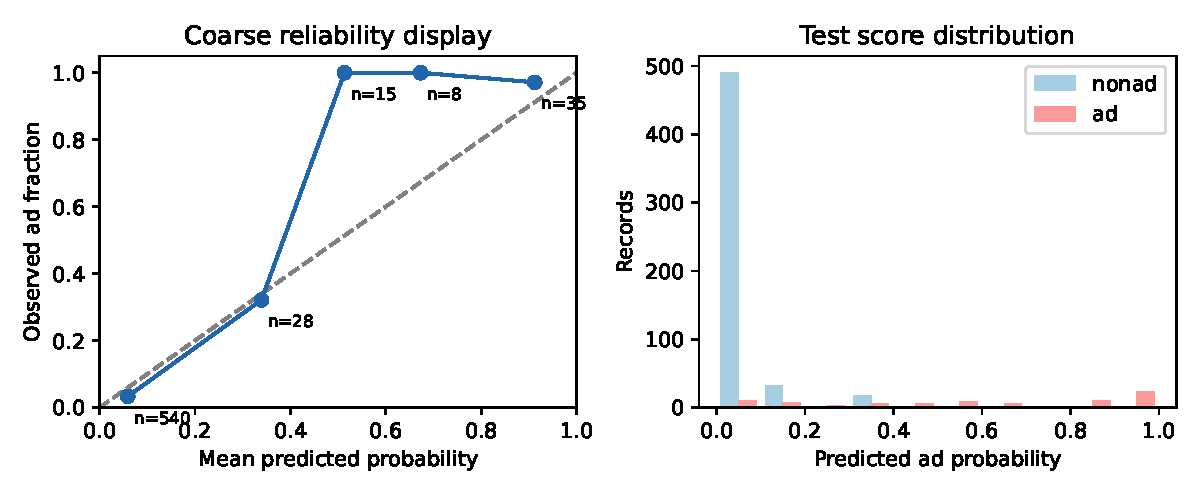
\includegraphics[width=\textwidth]{../analysis/results/reliability.pdf}
\caption{Post-evaluation probability assessment: reliability bins with record counts and the class-specific score distribution.}\label{fig:reliability}\end{figure}
Figure~\ref{fig:reliability} makes the bin sizes visible. The high observed fractions above score .4 suggest underprediction in those bins, but there are only 15, 8 and 35 records in the three upper bins. The lowest bin contains 540 records. Connecting bin averages is a descriptive display, not an estimated calibration function or an independent-sampling confidence statement. The histogram distinguishes concentrated low nonad scores from sparse high-score regions. No test-based recalibration is applied.
\section{Discussion, limitations, and extensions}
\subsection{Answers and strengths}
The first question is addressed descriptively by measured geometry differences and missingness: observed ad widths and aspect ratios are substantially larger, while missing geometry is more common among nonads. The second is answered by the held-out AP improvement of approximately 0.400 over geometry/locality and its paired conditional interval. The third is answered by the metric trade-off: full ridge leads on ranking, while the constrained tree leads on test F1 and Brier score. The fourth is answered by wide precision/F1 intervals and the limitations of the exchangeable-group approximation.

Keeping identical predictor patterns together reduces one identifiable source of optimistic evaluation. The separate validation partition keeps threshold selection out of the reported test calculation. Neither design choice explains the observed errors or establishes transfer to new websites. The ranking result is favorable, but threshold transfer is imperfect and the selected model is not best on every metric.

\subsection{Threats to validity}
\textbf{Representation and sampling.} The dataset describes an archival extracted representation, not contemporary pixels. Distinct patterns may come from the same website or template. The absent site identifiers prevent domain-held-out evaluation. The feature vocabulary itself was constructed before this study; the raw corpus is unavailable, so vocabulary-construction independence from evaluation examples cannot be verified. Splitting the supplied matrix cannot repair that upstream risk.

\textbf{Annotation and information loss.} Conflicting labels on identical features may reflect annotation errors or distinctions omitted by the representation. Neither explanation is established. Raw images and adjudication records would be needed. Context indicators may encode domain-specific shortcuts rather than broadly transferable advertisement characteristics.

\textbf{Missingness and preprocessing.} Median imputation is simple and reproducible but is not a model of the missing-data mechanism. Indicators allow availability-based prediction that may fail under changed extraction conditions. No imputation uncertainty is propagated into the predictive bootstrap. Log transforms impose a specific geometric scaling; sensitivity to that choice was not exhaustively studied.

\textbf{Selection and precision.} One fixed grouped split is not a study of training instability. A five-fold parameter search may overfit its CV criterion, and F1 tuning may exploit validation-specific composition. Reported test uncertainty holds those choices fixed. Tree complexity selection reaches a grid boundary, and no claim of algorithmic optimality follows. The test partition contains no conflicting-label group, which limits what it says about ambiguous representations.

\textbf{Interpretation.} Ridge coefficients should not be read as discoveries with ordinary confidence intervals. For example, \code{origurl*zdnet.com} has a large positive fitted coefficient, but rare terms, correlated indicators and standardization make a raw-coefficient ranking unsuitable as a general feature-importance ranking. Contextual features are predictive associations, not evidence that adding a phrase causes an image to become an ad.

\textbf{Population validity.} Confidence intervals rely on assumptions not secured by the source sampling documentation. Observed benchmark discrimination does not establish effectiveness for new domains, languages, rendering systems, or a new ad prevalence. AP, precision and F1 are particularly sensitive to prevalence and decision policy. The source's historical accuracy claim is not a comparable benchmark because its split and evaluation protocol differ.

\subsection{What would justify an action?}
On the fixed test sample, changing full ridge from .5 to the selected threshold recovers 16 additional ads but creates 24 additional false positives. Let $c_{FN}$ be the loss from a missed ad and $c_{FP}$ the loss from falsely blocking a nonad. The observed loss change is
\[L_{tuned}-L_{.5}=24c_{FP}-16c_{FN}.\]
The tuned policy has lower observed loss than .5 only when $c_{FP}/c_{FN}<2/3$. This retrospectively describes two already-reported policies; it is not a test-selected rule or population break-even estimate. It shows why F1 optimization can conflict with avoiding false blocking.

If $p$ were calibrated for deployment, predicting ad has conditional loss $c_{FP}(1-p)$ and predicting nonad has loss $c_{FN}p$. Minimum loss requires $p>c_{FP}/(c_{FP}+c_{FN})$. Neither those costs nor deployment-calibrated probabilities are available. The delivered output is a benchmark ranking with an illustrative binary operating point, not an asserted blocking policy.

\subsection{Targeted extensions}
The highest-value extension is a newly labeled collection with raw images, page/domain identifiers, extraction documentation, and an adjudication procedure. A domain-held-out test could then address template leakage, and a later collection could address temporal transfer. This would resolve a more important limitation than adding algorithms to the current split.

A deployment-oriented study should define false-blocking and missed-ad costs, use a new validation sample to select a cost-sensitive threshold, and investigate abstention for uncertain cases. Calibration should be fit on development data only and evaluated on a fresh test set. If estimating retraining variability becomes important, repeat grouped outer evaluation with inner tuning, while keeping domain groups intact when available. These extensions are proposals, not results already demonstrated.

\subsection{Final conclusion}
A regularized full-context classifier provides useful held-out ranking within the supplied Internet Advertisements benchmark. At the validation-selected operating point, test precision is 0.728 and recall is 0.798, with substantial uncertainty and a clear validation-to-test F1 decline. The defensible claim is improved benchmark discrimination over a geometry/locality comparator, not universal advertisement recognition or a ready-to-deploy blocking system.
\section{Data, code, and reproducibility sources}
\begin{itemize}
\item Original dataset and attribution: \url{https://archive.ics.uci.edu/dataset/51/internet+advertisements}; DOI \url{https://doi.org/10.24432/C5V011}. Repository license: CC BY 4.0.
\item Original downloadable files: \url{https://archive.ics.uci.edu/static/public/51/internet+advertisements.zip}. Copies of \code{ad.names}, \code{ad.DOCUMENTATION}, and \code{ad.data} are retained under \code{analysis/source/}.
\item Supplied analysis input: \href{../data/add.csv}{\code{data/add.csv}}; matched numerically and by label to the original source file.
\item Executed R code: \href{../analysis/run.R}{\code{analysis/run.R}}. Independent check: \href{../analysis/verify.py}{\code{analysis/verify.py}}. Public R source: \url{https://github.com/hlbathien/internet-advertisements-study/blob/main/analysis/run.R}. The repository contains the reproducible code and report sources.
\item Execution instructions: \href{../README.md}{\code{README.md}}. Split/fold assignments, test predictions, metric tables, model objects, and session record are under \code{analysis/results/}.
\end{itemize}
Run from the project root: \code{Rscript analysis/run.R}, then \code{python3 analysis/verify.py}. Regenerate the post-evaluation summaries and figures without fitting models:
\begin{quote}\small
\code{python3 analysis/critique_diagnostics.py}\\
\code{python3 analysis/plot_calibration.py}\\
\code{Rscript analysis/export_models.R}\\
\code{python3 analysis/render_tables.py}
\end{quote} R dependencies are \code{glmnet} and \code{rpart}; verification and plots use Python with NumPy, pandas, scikit-learn and Matplotlib. The executed R session used R 4.1.2, glmnet 4.1-3, rpart 4.1.16 and Matrix 1.4-0. Exact session details are saved in \code{analysis/results/sessionInfo.txt}. The PDF is built by running pdfLaTeX twice in \code{report/}. Absolute machine-specific input paths are not used by the analysis.

\section{References}
\small
\begin{enumerate}
\item Friedman, J., Hastie, T., and Tibshirani, R. \emph{An Introduction to glmnet}. Official glmnet documentation. \url{https://glmnet.stanford.edu/articles/glmnet.html}.
\item Kushmerick, N. (1999). \emph{Internet Advertisements} [Dataset]. UCI Machine Learning Repository. \url{https://doi.org/10.24432/C5V011}. Original accompanying files: \code{ad.DOCUMENTATION}, \code{ad.names}.
\item R Core / rpart documentation. \emph{Control for Rpart Fits}. \url{https://stat.ethz.ch/R-manual/R-devel/library/rpart/html/rpart.control.html}.
\item Scikit-learn developers. \emph{average\_precision\_score}. Official API documentation. \url{https://scikit-learn.org/stable/modules/generated/sklearn.metrics.average_precision_score.html}.
\end{enumerate}
\end{document}
